\pdfoutput=1
\pdfminorversion=7

\documentclass{article}


% if you need to pass options to natbib, use, e.g.:
\PassOptionsToPackage{numbers, compress}{natbib}
% before loading neurips_2025


% ready for submission
\usepackage{neurips_2025}
% \usepackage[preprint]{neurips_2025}
% to compile a preprint version, e.g., for submission to arXiv, add add the
% [preprint] option:



% to compile a camera-ready version, add the [final] option, e.g.:
    % \usepackage[final]{neurips_2025}


% to avoid loading the natbib package, add option nonatbib:
   % \usepackage[nonatbib]{neurips_2025}


\usepackage[utf8]{inputenc} % allow utf-8 input
\usepackage[T1]{fontenc}    % use 8-bit T1 fonts
\usepackage{hyperref}       % hyperlinks
\usepackage{url}            % simple URL typesetting
\usepackage{booktabs}       % professional-quality tables
\usepackage{amsfonts}       % blackboard math symbols
\usepackage{nicefrac}       % compact symbols for 1/2, etc.
\usepackage{microtype}      % microtypography
\usepackage{xcolor}         % colors

% \usepackage[table]{xcolor}         % colors
\usepackage{amsmath}
\usepackage{multirow}
% \usepackage{subfig}
\usepackage{tikz}
\usepackage{color}
\usepackage{pifont}
\usepackage{amssymb}
\usepackage{enumitem}
\usepackage{xspace}

\usepackage{graphicx}
\usepackage{caption} 
\usepackage{subcaption}
\usepackage{wrapfig}
\captionsetup[table]{skip=3pt}

\newcommand{\todo}[1]{\textcolor{red}{#1}}
\newcommand{\eg}{\textit{e.g.}} % for example
\newcommand{\ie}{\textit{i.e.}} % in other words
\newcommand{\yes}{\ding{51}}
\newcommand{\gyes}{\textcolor{black!30}{\ding{51}}}
\newcommand{\no}{\ding{55}}
\newcommand{\gno}{\textcolor{black!30}{\ding{55}}}

\newcommand{\etal}{\emph{et al.}}
\newcommand{\revision}[1]{\textcolor{black}{#1}}
\def\cf{\emph{c.f}\onedot} \def\Cf{\emph{C.f}\onedot}
\def\etc{\emph{etc}\onedot} \def\vs{\emph{vs}\onedot}
\def\wrt{w.r.t\onedot} \def\dof{d.o.f\onedot}
% \def\etal{\emph{et al}\onedot}
%
% --- inline annotations
%
\newcommand{\red}[1]{{\color{red}#1}}
\newcommand{\TODO}[1]{\textbf{\color{red}[TODO: #1]}}
% --- disable by uncommenting  
% \renewcommand{\TODO}[1]{}
% \renewcommand{\todo}[1]{#1}


\usepackage{graphicx}
\usepackage{amsmath}
\usepackage{amssymb}
\usepackage{booktabs}
\usepackage{adjustbox}
\usepackage{multirow}
\usepackage{arydshln}
\usepackage{colortbl}
% \usepackage{bookmark}
\usepackage{amsfonts}       % blackboard math symbols
\usepackage{nicefrac}       % compact symbols for 1/2, etc.
\usepackage{microtype}      % microtypography
\usepackage{times}
\usepackage{epsfig}
\usepackage{tipa}
\usepackage[T1, OT1]{fontenc}
\DeclareTextSymbolDefault{\dh}{T1}
\usepackage{booktabs}
\usepackage{multirow}
\usepackage{color, colortbl}
% \usepackage{subcaption}
\usepackage{pifont}
\usepackage{makecell}
% \usepackage{paralist}
\usepackage{threeparttable}
% \usepackage[shortlabels]{enumitem}
\usepackage{xcolor}
\usepackage{scalerel}
\usepackage{makecell}
\usepackage{tabu}
% \usepackage{hyperref}
\usepackage{tikz}
\usepackage{marvosym}
\usepackage{xcolor} 

\definecolor{Gray}{gray}{0.5}
\definecolor{LGray}{gray}{0.9}
\definecolor{darkblue}{RGB}{94,110,186}
\definecolor{darkGreen}{RGB}{92, 148, 110}
\definecolor{myblue}{RGB}{14, 121, 178}
\definecolor{rightpath}{RGB}{248, 203, 173}
\definecolor{wrongpath}{RGB}{89, 89, 89}


\newcommand{\cmark}{\ding{51}}%
\newcommand{\xmark}{\ding{55}}%

\newcommand{\darkGreen}[1]{\textcolor{darkGreen}{#1}}




\usepackage{tabulary}
\usepackage{tabulary,multirow,overpic,xcolor}
\newcolumntype{x}[1]{>{\centering\arraybackslash}m{#1pt}}
\newcolumntype{y}[1]{>{\arraybackslash}m{#1pt}}

\newcommand{\tablestyle}[2]{\setlength{\tabcolsep}{#1}\renewcommand{\arraystretch}{#2}\centering\footnotesize}
% \usepackage[colorlinks,linkcolor=black,bookmarks=false]{hyperref}
\title{StreamForest: Efficient Online Video Understanding with Persistent Event Memory}

\begin{document}


\appendix
% Section 编号为 A, B, C ...
\renewcommand{\thesection}{\Alph{section}}
% Subsection 编号为 A.1, A.2 ...
\renewcommand{\thesubsection}{\Alph{section}.\arabic{subsection}}

\section*{Appendix}
\addcontentsline{toc}{section}{Appendix}

Este apéndice proporciona información adicional para respaldar el texto principal. A continuación se presenta una tabla de contenidos para facilitar la navegación:

\begin{itemize}
    \item \hyperref[app:sec:Details_of_OnlineIT]{\textbf{A}}~\textbf{Detalles de OnlineIT}
    \begin{itemize}
        \item \hyperref[app:sec:Details_of_OnlineIT:OnlineIT-general]{A.1}~OnlineIT-general
        \item \hyperref[app:sec:Details_of_OnlineIT:OnlineIT-drive]{A.2}~OnlineIT-drive
    \end{itemize}

    \item \hyperref[app:sec:Details_of_ODVBench]{\textbf{B}}~\textbf{Detalles de ODV-Bench}
    \begin{itemize}
        \item \hyperref[app:sec:Details_of_ODVBench:Task]{B.1}~Taxonomía y formulación de tareas
        \item \hyperref[app:sec:Details_of_ODVBench:Statistics]{B.2}~Estadísticas del dataset
    \end{itemize}

    \item \hyperref[app:sec:More_Implementation_Details]{\textbf{C}}~\textbf{Más detalles de implementación}

    \item \hyperref[app:sec:Full_Performances]{\textbf{D}}~\textbf{Rendimientos completos}
    \begin{itemize}
        \item \hyperref[app:sec:Full_Performances:StreamingBench]{D.1}~StreamingBench
        \item \hyperref[app:sec:Full_Performances:OVBench]{D.2}~OVBench
        \item \hyperref[app:sec:Full_Performances:OVO-Bench]{D.3}~OVO-Bench
    \end{itemize}

    \item \hyperref[app:sec:Qualitative_Comparison]{\textbf{E}}~\textbf{Comparación cualitativa}

    \item \hyperref[app:sec:More_Ablations]{\textbf{F}}~\textbf{Más ablaciones}

    \item \hyperref[app:sec:Discussions]{\textbf{G}}~\textbf{Discusión}
    \begin{itemize}
        \item \hyperref[app:sec:Discussions:Limitations]{G.1}~Limitaciones
        \item \hyperref[app:sec:Discussions:Broader Impacts]{G.2}~Impactos más amplios
    \end{itemize}
\end{itemize}


\newpage


\section{Details of node's timestamp}
\label{app:sec:Details_of_node_timestamp}

Each event node's timestamp is initialized as the average time of the frames it represents (e.g., if an event node spans frames from 10s to 14s, its timestamp is initialized as 12s). When two event nodes are merged, the timestamp of the new node is computed as a token-count-weighted average of the original nodes:
\begin{equation}
t_{\text{new}} = \frac{t_i \cdot n_i + t_j \cdot n_j}{n_i + n_j},
\end{equation}
where $t_i$, $t_j$ are the timestamps of the original event nodes, and $n_i$, $n_j$ are the numbers of visual tokens contained in each node, respectively. This weighted scheme prevents timestamp drift during multiple rounds of merging, especially when the merged nodes contain significantly different amounts of visual tokens.

\section{Details of OnlineIT}
\label{app:sec:Details_of_OnlineIT}
In this section, we provide a comprehensive description of the task categorization and data distribution of the OnlineIT dataset. It is specifically designed to enhance the streaming video understanding capabilities of MLLMs in terms of real-time perception, future prediction, and event continuity. As shown in Table \ref{app:tab:OnlineIT}, the dataset is divided into two major components: OnlineIT-general, which targets general streaming video understanding, and OnlineIT-drive, which focuses on autonomous driving scenarios. Each subset is carefully designed to cover a diverse range of fine-grained perception and reasoning tasks with high-quality annotations.

\begin{table}[h]
    \centering
    \setlength{\tabcolsep}{3pt}
    \renewcommand{\arraystretch}{1.2}
    
    % 
    \caption{Task types and data volumes of OnlineIT.}
    
    \resizebox{0.9\textwidth}{!}{%
    
\begin{tabular}{ll|l|lr}
\hline
\rowcolor[HTML]{C0C0C0} 
\multicolumn{1}{l|}{Dataset} & Categories & Task & Sourse & Instance Num \\ \hline
\multicolumn{1}{c|}{\multirow{19}{*}{\rotatebox[origin=c]{90}{\footnotesize \textit{OnlineIT-general}}}} & \multirow{5}{*}{Spatial Perception} & \multirow{2}{*}{Spatial Grounding} & RefCOCO \cite{yu2016refcoco} & $\sim$43k \\
\multicolumn{1}{l|}{} &  &  & Allseeing-V2 \cite{wang2024allseeing_v2} & $\sim$45k \\ \cline{3-5} 
\multicolumn{1}{l|}{} &  & Multi-round Spatial Understanding & Visual Genome \cite{krishna2017vg} & $\sim$43k \\ \cline{3-5} 
\multicolumn{1}{l|}{} &  & Spatial Grounded VQA & Allseeing-V2 \cite{wang2024allseeing_v2} & $\sim$43k \\ \cline{3-5} 
\multicolumn{1}{l|}{} &  & Relative Spatial Localization & LaSOT \cite{fan2019lasot} & $\sim$19k \\ \cline{2-5} 
\multicolumn{1}{l|}{} & \multirow{5}{*}{Temporal Perception} & \multirow{3}{*}{Temporal Grounding} & Charades-STA \cite{charades-sta} & $\sim$11k \\
\multicolumn{1}{l|}{} &  &  & HiREST \cite{hirest} & $\sim$0.4k \\
\multicolumn{1}{l|}{} &  &  & QuerYD \cite{queryd} & $\sim$13k \\ \cline{3-5} 
\multicolumn{1}{l|}{} &  & Reasoning Temporal Localization & ActivityNet-RTL \cite{huang2024lita} & $\sim$10k \\ \cline{3-5} 
\multicolumn{1}{l|}{} &  & Multi-format Temporal Grounding & InternVid-VTime \cite{huang2024vtimellm} & $\sim$20k \\ \cline{2-5} 
\multicolumn{1}{l|}{} & \multirow{4}{*}{Spatiotemporal Perception} & Spatiotemporal Action Localization & AVA \cite{ava} & $\sim$6k \\ \cline{3-5} 
\multicolumn{1}{l|}{} &  & \multirow{2}{*}{Object Backward Tracking} & LaSOT \cite{fan2019lasot} & $\sim$51k \\
\multicolumn{1}{l|}{} &  &  & GOT \cite{got10k} & $\sim$58k \\ \cline{3-5} 
\multicolumn{1}{l|}{} &  & Spatiotemporal Detection & LaSOT \cite{fan2019lasot} & $\sim$14k \\ \cline{2-5} 
\multicolumn{1}{l|}{} & \multirow{5}{*}{Event Perception} & \multirow{3}{*}{Dense Video Captioning} & ActivityNet-Captions \cite{anet} & $\sim$10k \\
\multicolumn{1}{l|}{} &  &  & ViTT \cite{vitt} & $\sim$5k \\
\multicolumn{1}{l|}{} &  &  & Youcook2 \cite{youcook} & $\sim$1k \\ \cline{3-5} 
\multicolumn{1}{l|}{} &  & \multirow{2}{*}{Step Localization and Captioning} & COIN \cite{coin} & $\sim$9k \\
\multicolumn{1}{l|}{} &  &  & HiREST \cite{hirest} & $\sim$0.5k \\ \hline
\multicolumn{1}{c|}{\multirow{7}{*}{\rotatebox[origin=c]{90}{\footnotesize \textit{OnlineIT-drive}}}} & \multirow{3}{*}{Static Target} & Past Memory & D²-City \cite{che2019d} & $\sim$9k \\ \cline{3-5} 
\multicolumn{1}{l|}{} &  & \multirow{2}{*}{Real-time Perception} & TT100k \cite{zhu2016tt100k} & $\sim$46k \\
\multicolumn{1}{l|}{} &  &  & D²-City \cite{che2019d} & $\sim$13k \\ \cline{2-5} 
\multicolumn{1}{l|}{} & \multirow{2}{*}{Dynamic Target} & Localization Prediction & Road-waymo \cite{khan2024road} & $\sim$1k \\ \cline{3-5} 
\multicolumn{1}{l|}{} &  & Move Distance Prediction & Road-waymo \cite{khan2024road} & $\sim$7k \\ \cline{2-5} 
\multicolumn{1}{l|}{} & \multirow{2}{*}{Event Oriented} & Accident Reasoning & MM-AU \cite{fang2024abductive} & $\sim$6k \\ \cline{3-5} 
\multicolumn{1}{l|}{} &  & Risk Analysis & MM-AU \cite{fang2024abductive} & $\sim$7k \\ \hline 
\end{tabular}
        
    }
    
    \label{app:tab:OnlineIT}
\end{table}


\subsection{OnlineIT-general}
\label{app:sec:Details_of_OnlineIT:OnlineIT-general}
OnlineIT-general encompasses a broad scope of tasks designed to foster a comprehensive understanding of spatiotemporal video content in streaming settings. As shown in Table~\ref{app:tab:OnlineIT}, the dataset is categorized into four primary task types: spatial perception, temporal perception, spatiotemporal perception, and event perception. To ensure diversity, robustness, and fine-grained task coverage, we compiled and refined data from a wide array of sources. In total, OnlineIT-general comprises over 400k instances spanning various difficulty levels and video durations.

\paragraph{Spatial Perception.} This task type includes four subtasks. \textbf{\textit{Spatial Grounding}} requires the model to output the bounding box indicating the location of a queried object. \textbf{\textit{Multi-round Spatial Understanding}} involves identifying the object’s spatial location through multi-turn dialogue or generating a caption for the object within a specified spatial region. \textbf{\textit{Spatial Grounded VQA}} combines visual question answering with spatial localization, requiring the model to provide the bounding box of the relevant area while answering the question. \textbf{\textit{Relative Spatial Localization}} challenges the model to determine the position of a specified object relative to the overall scene. These tasks emphasize spatial grounding and reasoning, which are crucial for enhancing a model’s fine-grained spatial perception in real-time streaming video scenarios.

\paragraph{Temporal Perception.} This category consists of three subtasks. \textbf{\textit{Temporal Grounding}} involves interpreting a natural language query and identifying the start and end timestamps of the corresponding video segment. In streaming scenarios, the model must also assess whether the described event is currently ongoing. \textbf{\textit{Reasoning Temporal Localization}} requires identifying the relevant time span of an event while answering a reasoning-based question. \textbf{\textit{Multi-format Temporal Localization}} incorporates both single-turn and multi-turn dialogues, covering a diverse range of question formats. These tasks focus on strengthening the MLLM’s ability to track and reason about temporal dependencies, improving its understanding of both current and past moments in a video stream.

\paragraph{Spatiotemporal Perception.} This task type integrates spatial and temporal reasoning and includes three subtasks. \textbf{\textit{Spatiotemporal Action Localization}} requires the model to predict both the spatial location and the action being performed by a target at a specific query time. \textbf{\textit{Object Backward Tracking}} tasks the model with identifying the current location of an object and tracing its position at previous time points, such as one or two seconds earlier. \textbf{\textit{Spatiotemporal Detection}} operates over broader temporal windows, asking whether an object visible in the current frame existed several seconds ago or requiring the model to locate an object at a specified historical moment and determine its duration of existence. These tasks combine spatiotemporal cues to capture actions, motion, and transitions, allowing the model to track object trajectories and anticipate future states based on past and present context.

\paragraph{Event Perception.} This category includes two subtasks. \textbf{\textit{Dense Video Captioning}} involves detecting a sequence of events in a video and generating corresponding timestamps along with high-level descriptions. \textbf{\textit{Step Localization and Captioning}} differs by focusing on segmenting and narrating key procedural steps within long-form videos. These tasks are aimed at improving the model’s understanding of complex, multi-step events, enabling structured interpretation of dynamic sequences in streaming video understanding.


\subsection{OnlineIT-drive}
\label{app:sec:Details_of_OnlineIT:OnlineIT-drive}
OnlineIT-drive is designed specifically for the domain of streaming video understanding in autonomous driving. The dataset includes 89k instances, which are organized into three major task categories. Collectively, these tasks aim to strengthen not only real-time perception capabilities but also the temporal reasoning and decision-making abilities of MLLMs in high-stakes and rapidly evolving environments.

\paragraph{Static Target Understanding.}
To improve the model’s capacity for static scene understanding, two task types are introduced. \textit{\textbf{Real-time Perception}} requires the model to accurately perceive and interpret the semantics and spatial attributes of traffic-related targets as they appear in real time. \textit{\textbf{Past Memory}} assesses the model’s ability to retain and retrieve the semantics and spatiotemporal characteristics of traffic targets that were observed at a prior point in time. These tasks collectively enhance the model’s capability to perceive, understand, and remember static traffic elements and environmental context, such as road infrastructure and regulatory signage.

\paragraph{Dynamic Target Understanding.}
It includes two task types that aim to enhance predictive understanding of dynamic traffic participants. \textit{\textbf{Location Prediction}} requires the model to estimate the future position of a moving target based on its historical motion trajectory. \textit{\textbf{Move Distance Prediction}} focuses on predicting the distance traveled between the ego vehicle and other moving agents, given motion-related observations. These tasks are designed to improve the model’s ability to track continuously moving objects and to anticipate future trajectories.

\paragraph{Event Oriented Reasoning.}
It is intended to foster the development of reasoning abilities necessary for risk assessment and accident interpretation. \textit{\textbf{Risk Analysis}} requires the model to detect potential sources of danger in the current traffic scene and to assess the likelihood of accident occurrence. \textit{\textbf{Accident Reasoning}} involves post hoc analysis, where the model must infer the causes of an observed accident and articulate plausible preventive strategies. These tasks are designed to enhance the model’s ability to reason about causal relationships and to anticipate or reflect on traffic risks with contextual awareness.








\section{Details of ODV-Bench}
\label{app:sec:Details_of_ODVBench}


In this section, we detail the task taxonomy and formulation of the ODV-Bench, as well as the dataset statistics. We categorize task scenarios based on target entities and derive key perception and reasoning task types for each scenario in Table \ref{app:tab:task_templates}.

\begin{table*}[ht]
\centering
\renewcommand{\arraystretch}{1.25}

\caption{Resumen de las categorías de tareas, sus subcategorías y las plantillas de preguntas. }

\resizebox{\textwidth}{!}{
\begin{tabular}{ccl}
\hline
\rowcolor[HTML]{C0C0C0} 
Escenario objetivo de la tarea & Subtarea & Ejemplos de consultas \\
\hline


% -------- Static-target --------
\multicolumn{1}{c|}{} & \multicolumn{1}{c|}{\begin{tabular}[c]{@{}c@{}}Percepción de tránsito\\en tiempo real\end{tabular}} &
\begin{tabular}[c]{@{}l@{}}
1) \textquestiondown Cuál es el significado de la señal de tránsito en [0.61,0.31,0.64,0.38] en la imagen actual? \\
2) \textquestiondown Cuáles son las coordenadas de posición de la señal de tránsito que indica "Pedestrian Crossing" en la imagen actual? \\
3) \textquestiondown Cuál es el significado del cartel vial en [0.77,0.08,0.88,0.2] en la imagen actual? \\
4) Según el cartel vial en [0.09,0.46,0.19,0.52] en este momento, si vamos hacia la izquierda, \textquestiondown adónde iremos \\
y a qué distancia? \\
5) \textquestiondown Cuál es el color del semáforo en [0.42,0.01,0.45,0.13] en la imagen actual? Y \textquestiondown cuál es su indicación? \\
6) Según el cartel vial en [0.65,0.03,0.76,0.16] en este momento, \textquestiondown a qué distancia está Fengle?
\end{tabular} \\ \cline{2-3}

\multicolumn{1}{c|}{} & \multicolumn{1}{c|}{Memoria de tránsito pasada} &
\begin{tabular}[c]{@{}l@{}}
1) \textquestiondown Cuáles eran las coordenadas de posición de la señal de tránsito que indica "No Left Turn" en la escena hace 3 segundos? \\
2) \textquestiondown Cuál era el significado de la señal de tránsito en [0.39,0.13,0.41,0.17] en la escena hace 1 segundo? \\
3) La señal de tránsito se encuentra actualmente en [0.92,0.02,0.96,0.09]. \textquestiondown Cuáles eran sus coordenadas hace 2 segundos? \\
4) \textquestiondown Cuál era el color del semáforo en [0.35,0.1,0.38,0.22] en la escena hace 2 segundos?
\end{tabular} \\ \cline{2-3}

\multicolumn{1}{c|}{} & \multicolumn{1}{c|}{Toma de decisiones de conducción} &
\begin{tabular}[c]{@{}l@{}}
1) Según el cartel vial en [0.37,0.18,0.47,0.31] en la imagen tomada hace 2 segundos, si queremos ir a Renhe, \\
\textquestiondown en qué dirección debemos ir y a qué distancia está? \\
2) Según el cartel vial en [0.51,0.18,0.61,0.3] en este momento, si queremos ir a Libai Avenue, \textquestiondown en qué dirección\\
debemos ir y a qué distancia está? \\
3) Según el cartel vial en [0.38,0.04,0.63,0.23] en este momento, si queremos girar a la izquierda, \textquestiondown en qué carril deberíamos estar?
\end{tabular} \\ \cline{2-3}

\multicolumn{1}{c|}{} & \multicolumn{1}{c|}{Extracción de información clave} &
\begin{tabular}[c]{@{}l@{}}
1) Si queremos ir a Suzhou, \textquestiondown a qué objetivo deberíamos prestar más atención en este momento? \\
Indique el tipo y las coordenadas.
\end{tabular} \\ \cline{2-3}

\multicolumn{1}{c|}{} & \multicolumn{1}{c|}{Detección de alucinaciones} &
\begin{tabular}[c]{@{}l@{}}
1) Según el cartel vial en [0.38,0.31,0.52,0.48], \textquestiondown a qué distancia está actualmente Qingpu Town? \\
2) \textquestiondown Cuál es el significado de la señal de tránsito en [0.34,0.29,0.38,0.38] en la imagen actual? \\
3) \textquestiondown Cuál es el color del semáforo en [0.9,0.86,0.95,0.92] en la imagen actual?
\end{tabular} \\ \cline{2-3}


\multicolumn{1}{c|}{\multirow{-18}{*}{Objetivo estático}} & \multicolumn{1}{c|}{Detección de cambios de tránsito} &
\begin{tabular}[c]{@{}l@{}}
1) En el momento actual, \textquestiondown el semáforo que indica "turn right" más adelante se ha puesto completamente en verde? \\
2) En el momento actual, \textquestiondown el semáforo de adelante se ha puesto completamente en rojo? 
\end{tabular} \\
\hline

% -------- Dynamic-target --------
\multicolumn{1}{c|}{} & \multicolumn{1}{c|}{Predicción de acción} &
\begin{tabular}[c]{@{}l@{}}
1) \textquestiondown Cuál será el estado de movimiento posterior del automóvil ubicado actualmente en [0.993, 0.615, 1.0, 0.63]? 
\end{tabular} \\ \cline{2-3}

\multicolumn{1}{c|}{} & \multicolumn{1}{c|}{Predicción de ubicación} &
\begin{tabular}[c]{@{}l@{}}
1) \textquestiondown Cómo será el cuadro de posición del peatón ubicado en [0.544, 0.561, 0.613, 0.895] en el próximo segundo?
\end{tabular} \\ \cline{2-3}

\multicolumn{1}{c|}{\multirow{-3}{*}{Objetivo dinámico}} & \multicolumn{1}{c|}{Predicción de distancia} &
\begin{tabular}[c]{@{}l@{}}
1) \textquestiondown La distancia entre nuestro automóvil y el automóvil en [0.488, 0.488, 0.501, 0.494] se está haciendo mayor o menor?
\end{tabular} \\
\hline


% -------- Multi-agent Interaction Events --------
\multicolumn{1}{c|}{} & \multicolumn{1}{c|}{Predicción de riesgo} &
\begin{tabular}[c]{@{}l@{}}
1) \textquestiondown Existe una alta probabilidad de que ocurran accidentes de tránsito dentro de un cierto período en el futuro? \\
2) \textquestiondown Habrá riesgos de tránsito significativos dentro de un cierto período en el futuro? 
\end{tabular} \\ \cline{2-3}

\multicolumn{1}{c|}{} & \multicolumn{1}{c|}{Análisis de riesgo} &
\begin{tabular}[c]{@{}l@{}}
1) En este momento existe un alto riesgo de accidentes de tránsito. Según el entorno, \textquestiondown qué tipos de accidentes es probable que ocurran \\
y cuál es la base de esta predicción? \\
2) En este momento existen riesgos de tránsito significativos. Según el entorno, \textquestiondown cuáles son las fuentes de estos riesgos \\
y qué tipos de accidentes podrían causar?
\end{tabular} \\ \cline{2-3}

\multicolumn{1}{c|}{\multirow{-7}{*}{\begin{tabular}[c]{@{}c@{}}Evento de interacción\\ multiagente\end{tabular}}} 
& \multicolumn{1}{c|}{Respuesta sobre la causa del accidente} &
\begin{tabular}[c]{@{}l@{}}
1) \textquestiondown Cuál es la causa del accidente en el video? \textquestiondown Qué medidas pueden tomarse para evitarlo?
\end{tabular} \\ \hline

\end{tabular}%
}

\label{app:tab:task_templates}
\end{table*}


\subsection{Task Taxonomy and Formulation}
\label{app:sec:Details_of_ODVBench:Task}
We first identify the primary categories of traffic entities relevant to autonomous driving and organize task scenarios into three groups:\textbf{ (1) Tasks for Static Targets}, which involve the recognition and retrieval of stationary traffic elements such as traffic signs, lights, and road indicators; \textbf{ (2) Tasks for dynamic targets}, which focus on behavior prediction and localization of moving entities such as vehicles and pedestrians; and \textbf{ (3) Tasks for multitarget interaction events}, which capture complex interactions, risk scenarios, and accidents involving multiple agents. Based on these categories and guided by temporal cues and the practical needs of driving, we further define fine-grained task types to comprehensively assess model understanding in realistic online driving video scenarios.

\begin{figure*}[ht]
    \centering
    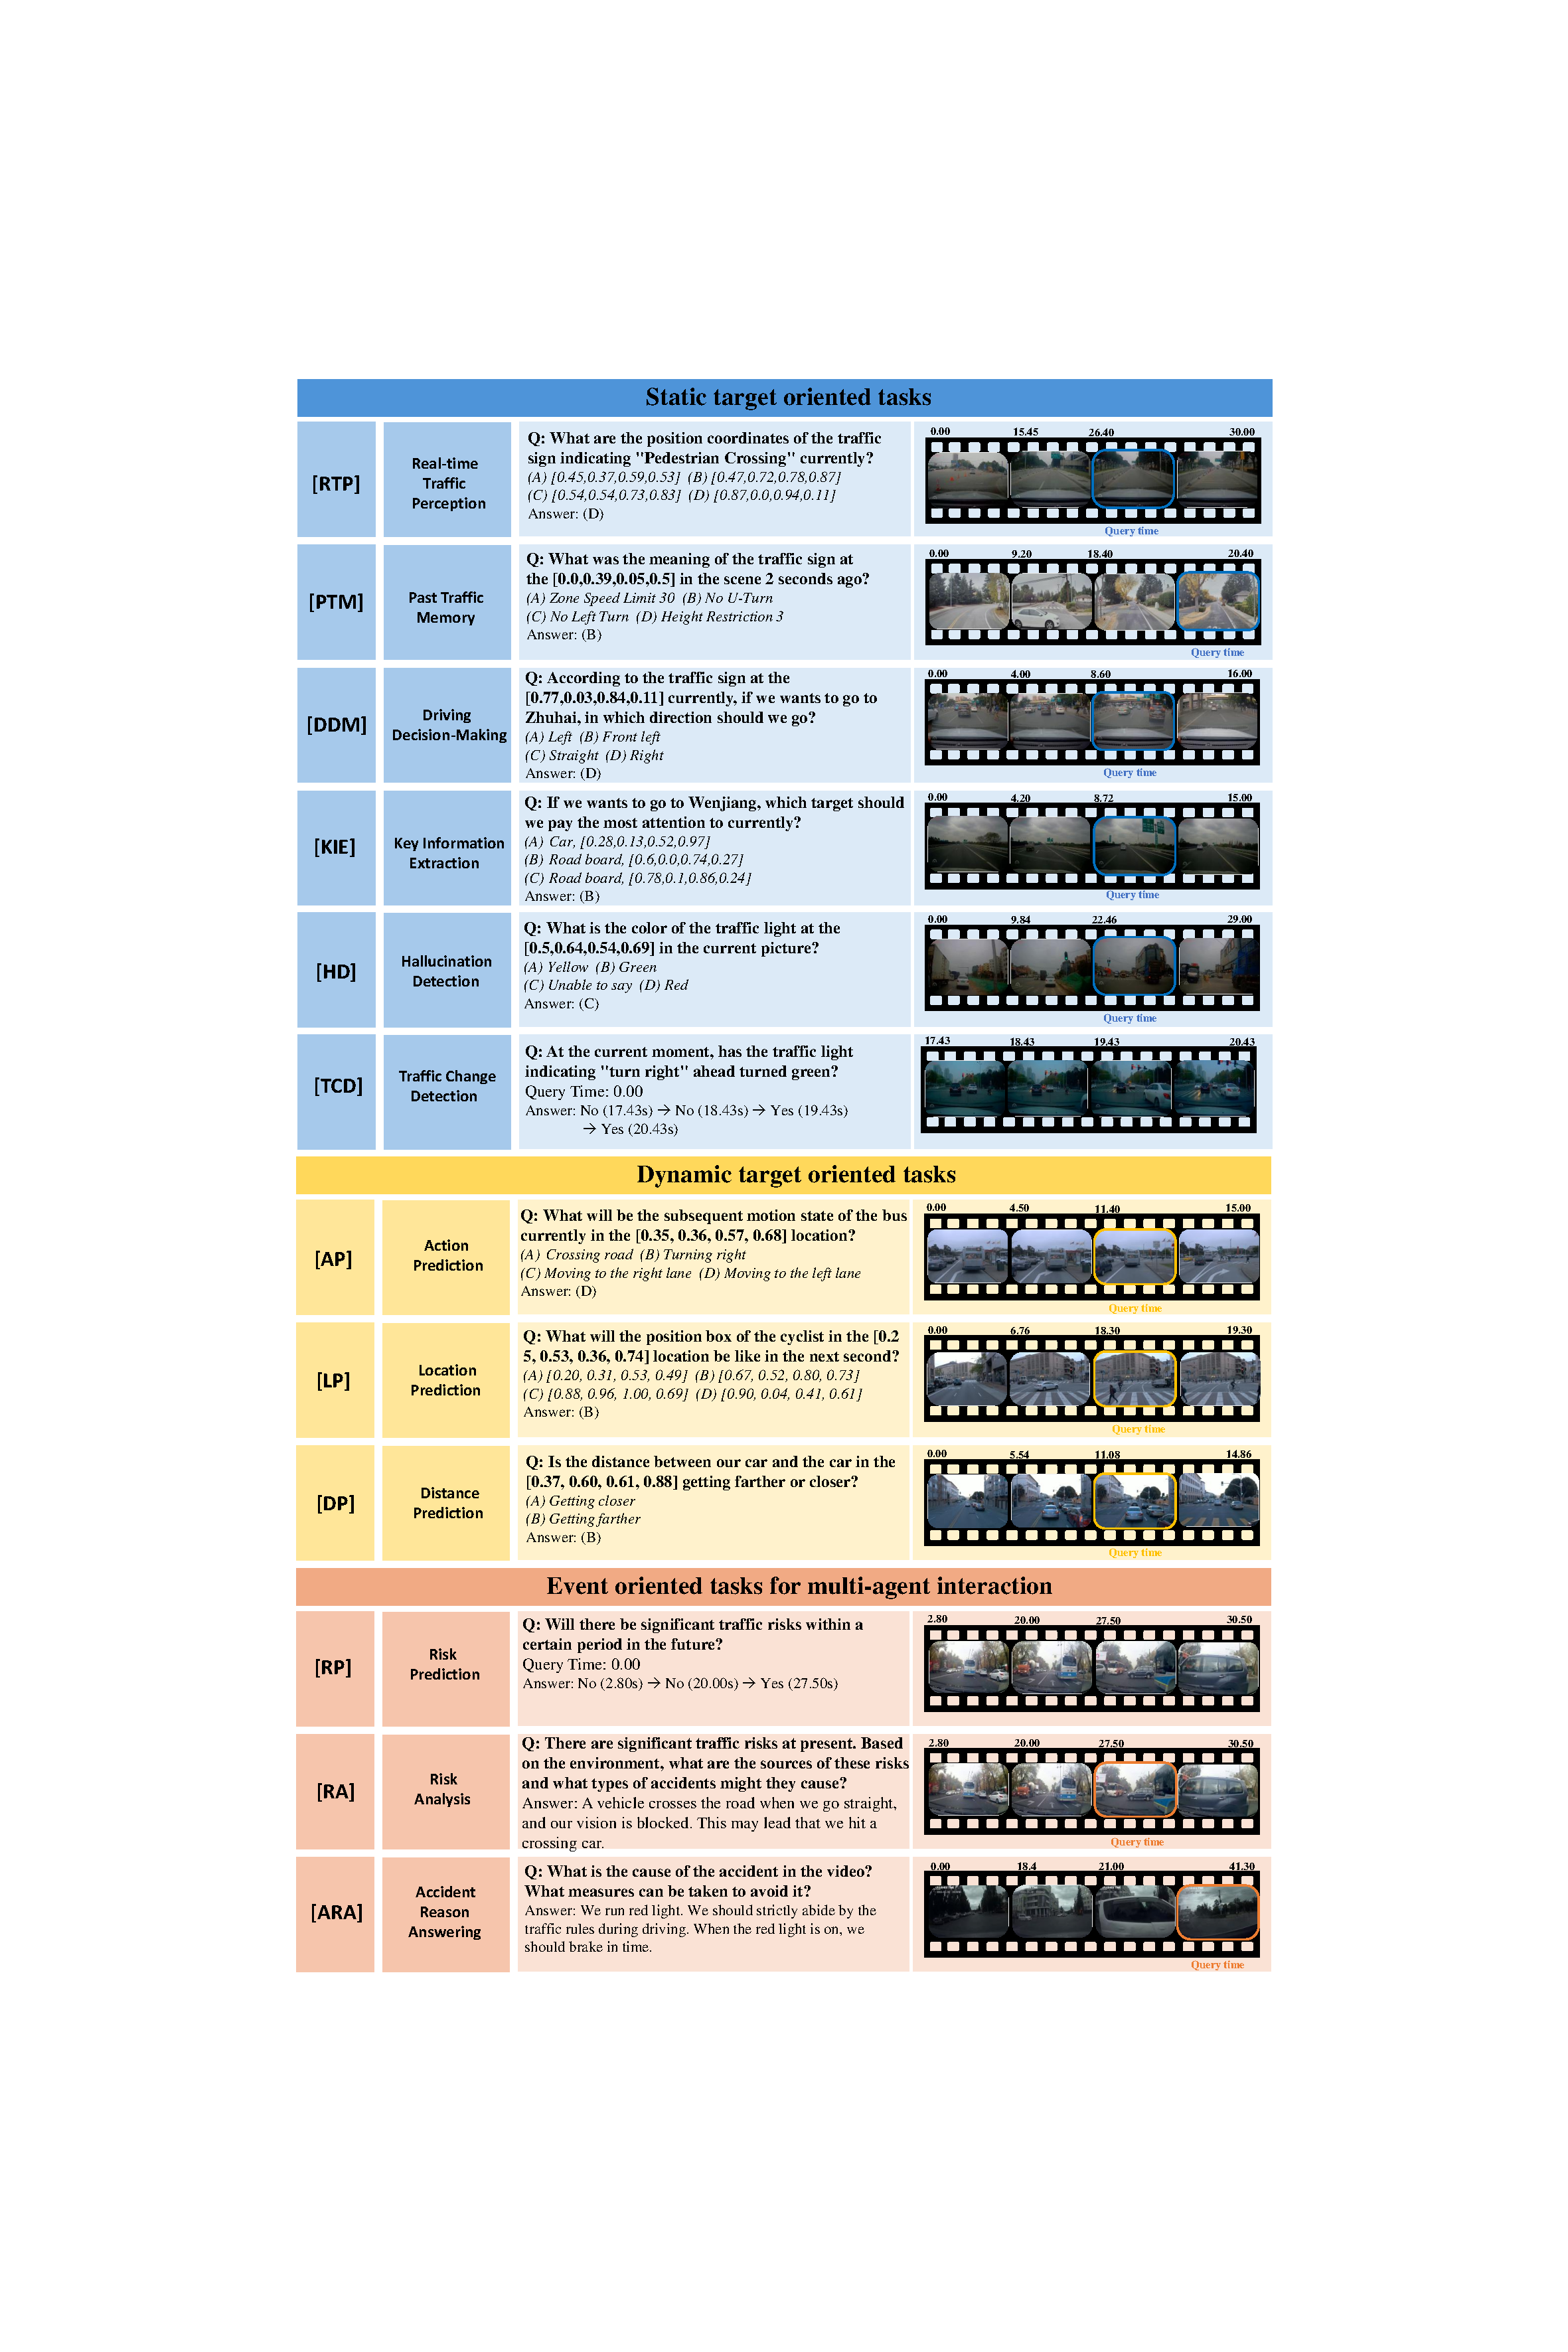
\includegraphics[width=0.8\textwidth]{figs/Appendix/odvbench_case_img.pdf} 
    \caption{Examples of each task in ODV-Bench. The 12 tasks are divided into three different perception modes for online video understanding for autonomous driving.
    }
    \label{app:fig:odvbench_case}
\end{figure*}

\subsubsection{Tasks for Static Targets}
Static traffic elements, such as traffic signs and road indicators, play a crucial role in driving decisions and hazard avoidance under normal driving conditions. To evaluate the model’s ability to retrieve and recognize these elements in online video streams, we design a dedicated set of tasks. Specifically, we distinguish between basic perception tasks and more advanced reasoning tasks, and further refine them based on temporal cues and practical driving needs: \textbf{(1) Real-time Traffic Perception:} Perceive and interpret the semantics and spatial locations of static traffic elements in real time; \textbf{(2) Past Traffic Memory:} Recall and track the semantics and spatiotemporal states of previously observed static elements; \textbf{(3) Driving Decision-Making:} make driving decisions based on the perceived information; \textbf{(4) Key Information Extraction:} Identify and locate key traffic elements critical to driving decisions; \textbf{(5) Hallucination Detection:} identify questions irrelevant to the existing video input; and \textbf{(6) Traffic Change Detection:} detect timestamps for changes in traffic elements, such as traffic lights.



\subsubsection{Tasks for Dynamic Targets}
The position and behavior of other road participants, such as vehicles and pedestrians, are crucial reference factors influencing autonomous driving decisions and safety. The ability to predict the position and behavior of dynamic traffic objects is essential to ensure the safety of autonomous driving. Therefore, we focus on the following three tasks to effectively evaluate this capability: \textbf{(1) Action Prediction:} predicting the next action of vehicles and pedestrians based on continuous spatiotemporal cues; \textbf{(2) Distance Prediction:} predicting the relative distance change between the ego-vehicle and other vehicles based on motion information; and \textbf{ (3) Location Prediction:} predicting the future spatial position of dynamic traffic targets based on their movement trajectories.


\subsubsection{Tasks for Multi-Target Interaction Events}
To achieve safe and reliable autonomous driving, the system must be able to identify risks and analyze accidents in complex road interaction scenarios. In the context of online video streams, this ability involves the dynamic recognition and analysis of multi-agent interactions, as well as the reasonable prediction of traffic risks. To evaluate this capability, we design the following three task categories: \textbf{(1) Risk Prediction:} predicting the occurrence of significant traffic risks and responding proactively; \textbf{(2) Risk Analysis:} detecting the sources of current traffic risks and analyzing the potential causes of accidents; and \textbf{ (3) Accident Reason Answering:} post-accident analysis, providing potential causes for the incident and summarizing actionable lessons learned.



\subsection{Dataset Statistics}
\label{app:sec:Details_of_ODVBench:Statistics}
ODV-Bench comprises 1,190 unique first-person driving video clips, encompassing a diverse range of driving scenarios across different countries from routine driving conditions to potential hazards and accidents. The length of videos ranges from 5 seconds to 90 seconds, effectively capturing the diversity of real-world streaming driving experiences. The benchmark includes 6,322 question-answer pairs, with an average query timestamp of 18.9 seconds. 
Specifically, the static-object-oriented category comprises 247 videos with a total of 1,639 questions; the dynamic-object-oriented category includes 162 videos and 2,973 questions; and the event-oriented category consists of 781 videos with 1,710 questions. All questions are in multiple-choice format, with the number of options varying between 2 and 4 depending on the question type.

























\section{More Implementation Details}
\label{app:sec:More_Implementation_Details}

\begin{table}[ht]
    \centering
    \setlength{\tabcolsep}{12pt}
    \renewcommand{\arraystretch}{1.2}
    
    % 
    \caption{Parameter settings for three-stage offline pre-training.}
    
    \resizebox{\textwidth}{!}{%
    
        \begin{tabular}{@{}ll|c|c|c@{}}
        \toprule
        & & \textbf{Stage-1}  & \textbf{Stage-2} & \textbf{Stage-3} \\ 
        \midrule 
        \multirow{2}{*}{\rotatebox[origin=c]{90}{\footnotesize \textit{Vision}}}
        & \textbf{Resolution$\times$Num. frames}  & 384 & 384$\times$8 & Max 384$\times$512  \\
        & \#Tokens & 64$\times$4  & 64$\times$8 & Max 16$\times$512   \\
        \midrule 
        \multirow{2}{*}{\rotatebox[origin=c]{90}{\footnotesize \textit{Data}}}
        & \textbf{Dataset} & Image \& Short Video & Image \& Short Video
        & Image \& Short / Long Video \\
        & \#Samples & 0.6M \& 0.5M & 3.8M \& 3.4M  & 0.5M \& 2.8M \\
        \midrule
        \multirow{2}{*}{\rotatebox[origin=c]{90}{\footnotesize \textit{Model}}}
        & \textbf{Trainable} & Projector & Full Model & Full Model  \\
        & \#parameters & 16.98MB & 8030.35MB & 8030.35MB \\
        \midrule 
        \multirow{4}{*}{\rotatebox[origin=c]{90}{\footnotesize \textit{Training}}}
        & \textbf{Batch Size} & 512 & 256 & 256  \\
        & \textbf{LR} of \textit{vision encoder} & 1$\times 10^{-3}$ & 2 $\times 10^{-6}$ & 2 $\times 10^{-6}$  \\    
        & \textbf{LR}\textit{ of connector \& LLM} & 1$\times 10^{-3}$ & 1 $\times 10^{-5}$ & 1 $\times 10^{-5}$   \\
        & \textbf{Epoch} & 1 & 1 & 1\\
        \bottomrule
        \end{tabular}
        
    }
    
    \label{app:tab:training_strategy_offline}
\end{table}

\begin{table}[ht]
    \centering
    \setlength{\tabcolsep}{12pt}
    \renewcommand{\arraystretch}{1.15}
    
    % 
    \caption{Parameter settings for the fourth stage online fine-tuning and fifth dirve fine-tuning.}
    
    \resizebox{0.8\textwidth}{!}{%
            
        \begin{tabular}{@{}ll|c|c@{}}
        \toprule
         &  & \textbf{Stage 4} & \textbf{Stage5} 
         \\ \midrule
         
        \multirow{3}{*}{\rotatebox[origin=c]{90}{\footnotesize \textit{Data}}} & \multirow{2}{*}{\textbf{Dataset}} & Image \& & Image \& 
        \\
        
         &  & (Short/Long/Online)-Video & (Short/Long/Online)-Video 
         \\
         
         & \#Samples & 0.4M \& 1.3M & 0.2M \& 0.5M
         \\ \midrule
         
        \multirow{2}{*}{\rotatebox[origin=c]{90}{\footnotesize \textit{Model}}} & \textbf{Trainable} & Projector \& LLM & Projector \& LLM
        \\
        
         & \#parameters & 7632.60MB & 7632.60MB 
         \\ \midrule
         
        \multirow{3}{*}{\rotatebox[origin=c]{90}{\footnotesize \textit{Vision}}} & \textbf{Resolution} & 384$\times$384 & 384$\times$384 
        \\
        
         & \textbf{Frames} & 2$\sim$512  & 2$\sim$512 
         \\
         
         & \textbf{FPS} & 1 & 1 
         \\ \midrule
         
        \multirow{6}{*}{\rotatebox[origin=c]{90}{\footnotesize \textit{Memory}}} & \textbf{Real-time Perception Qouta} & 729 & 729
        \\
        
         & \textbf{Spatiotemporal Memory Quota} & 128 $\times$ 18 & 128 $\times$ 18
         \\
         
         & \textbf{Total Visual Token Limits} & 8192 & 8192 
         \\
         
         & \textbf{Similarity Penalty Weight} & 0.4 & 0.4 
         \\
         
         & \textbf{Merge Count Penalty Weight} & 0.4 & 0.4 
         \\
         
         & \textbf{Temporal Distance Penalty Weight} & 0.2 & 0.2 
         \\ \midrule
         
        \multirow{9}{*}{\rotatebox[origin=c]{90}{\footnotesize \textit{Training}}} & \textbf{Batch Size} & 256 & 256 
        \\
        
         & \textbf{LR} & 1 $\times 10^{-5}$ & 1 $\times 10^{-5}$ 
         \\
         
         & \textbf{Epoch} & 1 & 1 
         \\
         
         & \textbf{Optimizer} & AdamW & AdamW
         \\
         
         & \textbf{Weight Decay} & 0 & 0
         \\
         
         & \textbf{Warmup Ratio} & 0.03 & 0.03 
         \\
         
         & \textbf{LR Schedule} & cosine & cosine 
         \\
         
         & \textbf{Vision Select Layer} & -2 & -2 
         \\
         
         & \textbf{GPU Nums} & 32 & 32
         \\ \bottomrule
         
        \end{tabular}
        
    }
    
    \label{app:tab:training_strategy_online}
\end{table}

We adopt a five-stage training strategy to systematically train the proposed StreamForest model, aiming to fully exploit its potential for streaming video understanding tasks. In the first three stages, we follow and extend the training paradigm of VideoChat-Flash \cite{li2024videochatflash}, employing offline training to endow the model with strong capabilities in long-form video comprehension and cross-modal alignment. These stages are designed progressively, covering diverse data scales and task objectives, enabling the model to gradually acquire core competencies such as basic vision-language alignment, long-term temporal modeling, and complex scene reasoning. Detailed training procedures and hyperparameter configurations for these stages are provided in Table~\ref{app:tab:training_strategy_offline}.




In the fourth and fifth stages, we perform online fine-tuning to enhance the model’s ability to process streaming inputs in realistic scenarios. By continuously feeding frame sequences during training, the model learns to retain a fine-grained perception of the current moment while maintaining long-term memory of past events, even under high compression constraints. The full configuration and parameter settings for the online fine-tuning phase are listed in Table~\ref{app:tab:training_strategy_online}. These stages are critical for transitioning the model from offline understanding to real-time reasoning, significantly improving its robustness and practical effectiveness in real-world applications.











\section{Full Performances}
\label{app:sec:Full_Performances}
In the following parts, we present the full results and compare StreamForest with leading proprietary and open-source models. To comprehensively evaluate the effectiveness of StreamForest, we conduct experiments on three online video understanding benchmarks: StreamingBench, OVBench, and OVO-Bench.

\subsection{StreamingBench}
\label{app:sec:Full_Performances:StreamingBench}
% Please add the following required packages to your document preamble:
% \usepackage{graphicx}
% \usepackage[table,xcdraw]{xcolor}
% Beamer presentation requires \usepackage{colortbl} instead of \usepackage[table,xcdraw]{xcolor}
\begin{table}[ht]
\setlength{\tabcolsep}{3pt}
\renewcommand{\arraystretch}{1.1}
\centering

\caption{Resultados completos de evaluación de tareas de comprensión en tiempo real en StreamingBench.}

\resizebox{0.75\textwidth}{!}{%
\begin{tabular}{lccccccccccccc}
\midrule\midrule
{Method}             & {Size} & \multicolumn{1}{l|}{{\#Frames}} & {OP}                  & {CR}                  & {CS}                  & {ATP}                 & {EU}                  & {TR}                  & {PR}                  & {SU}                  & {ACP}                 & \multicolumn{1}{c|}{{CT}}                  & {ALL}                 \\ \midrule
Human                       & -             & \multicolumn{1}{c|}{-}                 & 89.47                        & 92.00                        & 93.60                        & 91.47                        & 95.65                        & 92.52                        & 88.00                        & 88.75                        & 89.74                        & \multicolumn{1}{c|}{91.30}                        & 91.46                        \\ \midrule
\multicolumn{14}{l}{\textit{Proprietary MLLMs}} \\ \midrule
Gemini 1.5 pro \cite{team2024gemini}             & -             & \multicolumn{1}{c|}{1fps}              & 79.02                        & 80.47                        & 83.54                        & 79.67                        & 80.00                        & 84.74                        & 77.78                        & 64.23                        & 71.95                        & \multicolumn{1}{c|}{48.70}                        & 75.69                        \\
GPT-4o  \cite{openai2024gpt4o}                    & -             & \multicolumn{1}{c|}{64}                & { 77.11} & { 80.47} & { 83.91} & { 76.47} & { 70.19} & { 83.80} & { 66.67} & { 62.19} & { 69.12} & \multicolumn{1}{c|}{{ 49.22}} & { 73.28} \\
Claude 3.5 Sonnet \cite{claude3_5}          & -             & \multicolumn{1}{c|}{20}                & { 73.33} & { 80.47} & { 84.09} & { 82.02} & { 75.39} & { 79.53} & { 61.11} & { 61.79} & { 69.32} & \multicolumn{1}{c|}{{ 43.09}} & { 72.44} \\ \midrule
\multicolumn{14}{l}{\textit{Open-source Offline Video MLLMs}}                                                                                                                                                                                                                                                                                                                                                                                                  \\ \midrule
Video-LLaMA2    \cite{cheng2024videollama2}            & 7B            & \multicolumn{1}{c|}{32}                & 55.86                        & 55.47                        & 57.41                        & 58.17                        & 52.80                        & 43.61                        & 39.81                        & 42.68                        & 45.61                        & \multicolumn{1}{c|}{35.23}                        & 49.52                        \\
VILA-1.5   \cite{lin2024vila}                 & 8B            & \multicolumn{1}{c|}{14}                & 53.68                        & 49.22                        & 70.98                        & 56.86                        & 53.42                        & 53.89                        & 54.63                        & 48.78                        & 50.14                        & \multicolumn{1}{c|}{17.62}                        & 52.32                        \\
Video-CCAM  \cite{fei2024videoccam}                & 14B           & \multicolumn{1}{c|}{96}                & 56.40                        & 57.81                        & 65.30                        & 62.75                        & 64.60                        & 51.40                        & 42.59                        & 47.97                        & 49.58                        & \multicolumn{1}{c|}{31.61}                        & 53.96                        \\
LongVA   \cite{zhang2024longva}                   & 7B            & \multicolumn{1}{c|}{128}               & 70.03                        & 63.28                        & 61.20                        & 70.92                        & 62.73                        & 59.50                        & 61.11                        & 53.66                        & 54.67                        & \multicolumn{1}{c|}{34.72}                        & 59.96                        \\
InternVL2 \cite{chen2024internvl2}                & 8B            & \multicolumn{1}{c|}{16}                & 68.12                        & 60.94                        & 69.40                        & 77.12                        & 67.70                        & 62.93                        & 59.26                        & 53.25                        & 54.96                        & \multicolumn{1}{c|}{56.48}                        & 63.72                        \\
Kangaroo   \cite{liu2024kangaroo}                 & 7B            & \multicolumn{1}{c|}{64}                & 71.12                        & 84.38                        & 70.66                        & 73.20                        & 67.08                        & 61.68                        & 56.48                        & 55.69                        & 62.04                        & \multicolumn{1}{c|}{38.86}                        & 64.60                        \\
LLaVA-NeXT-Video    \cite{zhang2024llavavideo}        & 32B           & \multicolumn{1}{c|}{64}                & 78.20                        & 70.31                        & 73.82                        & 76.80                        & 63.35                        & 69.78                        & 57.41                        & 56.10                        & 64.31                        & \multicolumn{1}{c|}{38.86}                        & 66.96                        \\
MiniCPM-V2.6   \cite{yao2024minicpmv}             & 8B            & \multicolumn{1}{c|}{32}                & 71.93                        & 71.09                        & 77.92                        & 75.82                        & 64.60                        & 65.73                        & 70.37                        & 56.10                        & 62.32                        & \multicolumn{1}{c|}{53.37}                        & 67.44                        \\
LLaVA-OneVision   \cite{li2024llavaov}          & 7B            & \multicolumn{1}{c|}{32}                & 80.38                        & 74.22                        & 76.03                        & 80.72                        & 72.67                        & 71.65                        & 67.59                        & 65.45                        & 65.72                        & \multicolumn{1}{c|}{45.08}                        & 71.12                        \\
Qwen2.5-VL   \cite{bai2025qwen2_5vl}               & 7B            & \multicolumn{1}{c|}{1fps}              & 78.32                        & 80.47                        & 78.86                        & 80.45                        & 76.73                        & 78.50                        & 79.63                        & 63.41                        & 66.19                        & \multicolumn{1}{c|}{53.19}                        & 73.68                        \\ \midrule
\multicolumn{14}{l}{\textit{Open-source Online Video MLLMs}}                                                                                                                                                                                                                                                                                                                                                                                                   \\ \midrule
Flash-VStream   \cite{zhang2024flashvstream}            & 7B            & \multicolumn{1}{c|}{-}                 & 25.89                        & 43.57                        & 24.91                        & 23.87                        & 27.33                        & 13.08                        & 18.52                        & 25.20                        & 23.87                        & \multicolumn{1}{c|}{48.70}                        & 23.23                        \\
VideoLLM-online \cite{chen2024videollmonline}            & 8B            & \multicolumn{1}{c|}{2fps}              & 39.07                        & 40.06                        & 34.49                        & 31.05                        & 45.96                        & 32.40                        & 31.48                        & 34.16                        & 42.49                        & \multicolumn{1}{c|}{27.89}                        & 35.99                        \\
Dispider \cite{qian2025dispider}                   & 7B            & \multicolumn{1}{c|}{1fps}              & 74.92                        & 75.53                        & 74.10                        & 73.08                        & 74.44                        & 59.92                        & 76.14                        & 62.91                        & 62.16                        & \multicolumn{1}{c|}{45.80}                        & 67.63                        \\
% TimeChat-Online             & 7B            & \multicolumn{1}{c|}{1fps}              & 80.22                        & 82.03                        & 79.50                        & 83.33                        & 76.10                        & 78.50                        & 78.70                        & 64.63                        & 69.60                        & \multicolumn{1}{c|}{57.98}                        & 75.36                        \\ 
\midrule
\textbf{StreamForest(Ours)} & {7B}   & \multicolumn{1}{c|}{{1fps}}     & 83.11                        & 82.81                        & 82.65                        & 84.26                        & 77.50                        & 78.19                        & 76.85                        & 69.11                        & 75.64                        & \multicolumn{1}{c|}{54.40}                        & 77.26                        \\  \midrule\midrule
\end{tabular}%
}

\label{app:tab:streamingbench}

\end{table}


Table~\ref{app:tab:streamingbench} presents the full evaluation results on StreamingBench, covering 12 real-time video understanding tasks. StreamForest achieves the highest average score (77.26\%) among all evaluated models, both open-source and proprietary, while operating efficiently at 1 fps. Notably, StreamForest outperforms leading proprietary MLLMs such as GPT-4o (73.28\%) and Gemini 1.5 Pro (75.69\%). It also significantly surpasses top open-source offline models such as LLaVA-OneVision (71.12\%) and Qwen2.5-VL (73.68\%), underscoring its robust multimodal representation and reasoning capabilities. In the online video MLLM category, StreamForest sets a new state-of-the-art, outperforming open-source counterparts Dispider (67.63\%) by a wide margin. Its consistent accuracy and real-time efficiency demonstrate a strong potential for practical deployment in streaming applications.

\subsection{OVBench}
\label{app:sec:Full_Performances:OVBench}
%usepackage{adjustbox}
\begin{table*}[ht]
    \centering
    % \renewcommand{\arraystretch}{1.1}

    \caption{Resultados completos de evaluación en OVBench.}


    
    \resizebox{\textwidth}{!}{%
    \begin{tabular}{lc|cccccccccccccccc|c}
        \toprule \toprule 
        Task   Name                 &                                      & \multicolumn{3}{c}{FP}                                                  & \multicolumn{3}{c}{THV}                                                    & \multicolumn{3}{c}{PM}                                                  & \multicolumn{2}{c}{SP}                        & \multicolumn{2}{c}{STP}                         & \multicolumn{3}{c|}{TP}                                                  &                       \\
        \cmidrule(lr){3-5} \cmidrule(lr){6-8} \cmidrule(lr){9-11} \cmidrule(lr){12-13} \cmidrule(lr){14-15} \cmidrule(lr){16-18}
        Subset Name                 & {\multirow{-2}{*}{Size}}           & AA & GSP & MP & AP & SV & OP & AR & PR & TR & AL & OP & AT & OT & AS & SL & OES & {\multirow{-2}{*}{AVG}} \\
        \midrule
        \multicolumn{19}{l}{\textit{Proprietary MLLMs}}                                   \\
        \midrule
        Gemini-1.5-Flash~\cite{team2024gemini}           & -                                    & 71.4                  & 53.6                    & 21.9                  & 56.5                   & 60.8                     & 40.6                   & 36.7                  & 47.9                    & 62.5                  & 32.3                  & 37.5                  & 87.0                   & 50.0                   & 83.3                  & 22.3                    & 46.9                  & 50.7                                      \\
        \midrule
        \multicolumn{19}{l}{\textit{Open-source Offline Video MLLMs}}                                   \\ 
        \midrule
        InternVL2~\cite{chen2024internvl2}                   & 7B                                                       & 52.6                  & 60.2                    & 27.6                  & 57.5                   & {52.0}                     & 58.5                   & {38.8}                  & 67.1                    & 58.3                  & 38.1                  & 31.3                  & 87.4                   & 37.0                   & {75.4}                  & {31.4}                    & 5.9                   & 48.7                                      \\
        InternVL2~\cite{chen2024internvl2}                   & 4B                                                       & 57.7                  & 57.0                    & 14.4                  & 59.2                  & 49.4                     & {60.0}                   & 30.3                  & 61.8                    & 46.3                  & 30.9                  & 20.1                  & 83.0                   & 32.3                   & 70.7                  & 29.4                    & 3.4                   & 44.1                                      \\
        LLaMA-VID~\cite{li2024llamavid}                   & 7B                                                       & 43.6                  & 50.9                    & 19.6                  & {64.0}                   & 47.5                     & 46.8                   & 29.4                  & 48.9                    & 51.2                  & 31.9                  & 11.2                  & 75.7                   & 24.8                   & 59.1                  & 26.0                    & {40.0}                  & 41.9                                      \\
        LLaVA-Onevision~\cite{li2024llavaov}             & 7B                                                       & 68.0                  & 62.7                    & 35.9                  & 58.4                   & 50.3                     & 46.5                   & 29.4                  & 60.7                    & 58.0                  & 43.1                  & 14.2                  & 86.5                   & {49.7}                   & 70.7                  & 28.1                    & 30.2                  & 49.5                                      \\
        LongVA~\cite{zhang2024longva}                        & 7B                                                       & 64.1                  & 56.5                    & {29.5}                  & 54.9                   & 51.9                     & 34.8                   & 35.3                  & 55.6                    & 57.7                  & 31.6                  & 3.4                   & 67.4                   & 44.7                   & 80.0                  & 26.7                    & 4.0                   & 43.6                                      \\
        MiniCPM-V2.6~\cite{yao2024minicpmv}                & 7B                                                       & 33.3                  & 35.9                    & 15.0                  & 59.2                   & 50.8                     & 55.1                   & 25.0                  & 37.4                    & 41.7                  & 26.6                  & 11.8                  & 98.3                   & 36.3                   & 66.1                  & 26.4                    & 6.2                   & 39.1                                      \\
        Qwen2-VL~\cite{qwen2vl}                   & 7B                                                       & {60.3}                  & 66.1                   & 22.1                  & 54.9                   & 51.5                     & 51.1                   & 37.8                  & {64.4}                    & {69.3}                  & 35.3                  & 28.5                  & {97.0}                   & 49.4                   & 65.1                  & 30.8                    & 11.7                  & {49.7}                                      \\
        {LITA}~\cite{huang2024lita}                          & 7B                                                       &19.2	&24.5	&19.9	&40.8	&48.9	&24.9	&3.1	&27.3	&6.4	&6.9	&14.6	&35.2	&23.9	&27.4	&0.5	&3.4	&20.4
    
                         \\
        {TimeChat}~\cite{ren2024timechat}                    & 7B                                                       &7.7	&15.3	&18.7	&20.6	&15.7	&11.7	&9.1	&14.7	&9.8	&7.5	&19.5	&13.9	&10.3	&9.3	&10.1	&10.8	&12.8
                         \\
        VTimeLLM~\cite{huang2024vtimellm}                    & 7B                                                       & 37.2                  & 23.4                    & 15.0                  & 64.8                   & 43.8                     & 53.2                   & 25.9                  & 38.8                 & 32.5                  & 25.9                  & 20.4                  & 40.9                   & 6.8                    & 48.4                  & 43.5                    & 8.6                   & 33.1                                      \\
        \midrule
        \multicolumn{19}{l}{\textit{Open-source Online Video MLLMs}}                         \\
        \midrule
        {VideoLLM-Online}~\cite{chen2024videollmonline}               & 7B                                                       &0	&1.8	&20.9	&5.2	&5.9	&32.6	&0	&2.3	&26.7	&0.6	&26.6	&0.9	&19.9	&0.9	&1.7	&8.3	&9.6
                         \\
        MovieChat~\cite{song2024moviechat}                   & 7B                                                       & 23.1                  & 27.5                    & 23.6                  & 58.4                   & 43.9                     & 40.3                   & 25.6                  & 31.1                    & 23.9                  & 26.9                  & 39.6                  & 24.4                   & 28.9                   & 29.3                  & 25.5                    & 21.9                  & 30.9                                      \\
        Flash-Vstream~\cite{zhang2024flashvstream}                 & 7B                                                       & 26.9                  & 37.6                    & 23.9                  & 60.1                   & 41.9                     & 40.0                   & 23.4                  & 35.3                    & 26.1                  & 24.7                  & 28.8                  & 27.0                   & 21.4                   & 29.8                  & 25.6                    & 26.8                  & 31.2                                      \\
        Videochat-Online~\cite{huang2024videochatonline}                        & 4B                                                       & 64.1                  & 59.7                  & 16.6                  & 63.1                   & 58.3                     & 62.8                   & 42.2                  & 54.4                    & 70.6                  & 54.1                  & 24.8                  & 88.7                   & 48.5                   & 73.0                  & 25.9                    & 71.7                  & 54.9                                      \\ \midrule 
        \textbf{StreamForest (Ours)}                       & {7B}                                                       & {69.2}                  & {60.0}                  & {34.4}                  & {69.1}                   & {54.0}                     & {72.9}                   & {50.9}                  & {64.9}                    & {82.2}                  & {56.6}                  & {87.9}                  & {95.2}                   & {61.2}                   & {64.2}                  & {30.6}                    & {92.6}                  & {60.5}                                      \\
        
    
    \bottomrule \bottomrule
    
    \end{tabular}%
    }


\label{app:tab:ov_bench}
    \end{table*}


Table~\ref{app:tab:ov_bench} shows the comprehensive results on OVBench, encompassing six diverse task categories (FP, THV, PM, SP, STP, TP). StreamForest achieves the top average score of 60.5\%, surpassing all open-source online and offline Video MLLMs. It significantly outperforms other open-source online models, e.g., Videochat-Online (54.9\%) and Flash-VStream (31.2\%), as well as offline models such as Qwen2-VL (49.7\%) and LLaVA-OneVision (49.5\%). Compared to Gemini-1.5-Flash (50.7\%), StreamForest delivers nearly 10 points higher accuracy on average, affirming its capability to balance real-time efficiency with high performance.

\subsection{OVO-Bench}
\label{app:sec:Full_Performances:OVO-Bench}
\begin{table*}[ht]
    \centering
    \renewcommand{\arraystretch}{1.1}  % Increase row spacing
    
        \caption{{Resultados detallados de evaluación en OVO-Bench.}}
        
    \resizebox{1.0\textwidth}{!}{%
        \begin{tabular}{lccccccccccccccccc}
            \midrule\midrule
            \multicolumn{1}{c|}{} &
              \multicolumn{1}{l|}{} &
              \multicolumn{7}{c|}{{Real-Time Visual Perception}} &
              \multicolumn{4}{c|}{{Backward Tracing}} &
              \multicolumn{4}{c|}{{Forward Active Responding}} &
             \\ \cmidrule{3-17} 
            \multicolumn{1}{c|}{\multirow{-2}{*}{{Model}}} &
              \multicolumn{1}{l|}{\multirow{-2}{*}{{\# Frames}}} &
              OCR &
              ACR &
              ATR &
              STU &
              FPD &
              \multicolumn{1}{c|}{OJR} &
              \multicolumn{1}{c|}{Avg.} &
              EPM &
              ASI &
              \multicolumn{1}{c|}{HLD} &
              \multicolumn{1}{c|}{Avg.} &
              REC &
              SSR &
              \multicolumn{1}{c|}{CRR} &
              \multicolumn{1}{c|}{Avg.} &
              \multirow{-2}{*}{Overall Avg.} \\ \midrule
            \multicolumn{1}{l|}{Human} &
              \multicolumn{1}{c|}{-} &
              93.96 &
              92.57 &
              94.83 &
              92.70 &
              91.09 &
              \multicolumn{1}{c|}{94.02} &
              \multicolumn{1}{c|}{93.20} &
              92.59 &
              93.02 &
              \multicolumn{1}{c|}{91.37} &
              \multicolumn{1}{c|}{92.33} &
              95.48 &
              89.67 &
              \multicolumn{1}{c|}{93.56} &
              \multicolumn{1}{c|}{92.90} &
              92.81 \\ \midrule
            \multicolumn{18}{l}{\textit{Proprietary MLLMs}} \\ \midrule
            \multicolumn{1}{l|}{Gemini 1.5 Pro \cite{team2024gemini}} &
              \multicolumn{1}{c|}{1fps} &
              {85.91} &
              {66.97} &
              {79.31} &
              {58.43} &
              63.37 &
              \multicolumn{1}{c|}{{61.96}} &
              \multicolumn{1}{c|}{{69.32}} &
              {58.59} &
              {76.35} &
              \multicolumn{1}{c|}{{52.64}} &
              \multicolumn{1}{c|}{{62.54}} &
              {35.53} &
              {74.24} &
              \multicolumn{1}{c|}{{61.67}} &
              \multicolumn{1}{c|}{{57.15}} &
              {63.00} \\
            \multicolumn{1}{l|}{GPT-4o \cite{openai2024gpt4o}} &
              \multicolumn{1}{c|}{64} &
              69.80 &
              64.22 &
              71.55 &
              51.12 &
              {70.30} &
              \multicolumn{1}{c|}{59.78} &
              \multicolumn{1}{c|}{64.46} &
              57.91 &
              75.68 &
              \multicolumn{1}{c|}{48.66} &
              \multicolumn{1}{c|}{60.75} &
              27.58 &
              73.21 &
              \multicolumn{1}{c|}{59.40} &
              \multicolumn{1}{c|}{53.40} &
              59.54 \\ \midrule
            \multicolumn{18}{l}{\textit{Open-source Offline Video MLLMs}} \\ \midrule
            \multicolumn{1}{l|}{LLaVA-Video-7B \cite{zhang2024llavavideo}} &
              \multicolumn{1}{c|}{64} &
              69.80 &
              59.63 &
              66.38 &
              50.56 &
              72.28 &
              \multicolumn{1}{c|}{61.41} &
              \multicolumn{1}{c|}{63.34} &
              51.18 &
              64.19 &
              \multicolumn{1}{c|}{9.68} &
              \multicolumn{1}{c|}{41.68} &
              34.10 &
              {67.57} &
              \multicolumn{1}{c|}{60.83} &
              \multicolumn{1}{c|}{{54.17}} &
              53.06 \\
            \multicolumn{1}{l|}{LLaVA-OneVision-7B \cite{li2024llavaov}} &
              \multicolumn{1}{c|}{64} &
              67.11 &
              58.72 &
              69.83 &
              49.44 &
              71.29 &
              \multicolumn{1}{c|}{60.33} &
              \multicolumn{1}{c|}{62.79} &
              52.53 &
              58.78 &
              \multicolumn{1}{c|}{23.66} &
              \multicolumn{1}{c|}{44.99} &
              24.79 &
              66.93 &
              \multicolumn{1}{c|}{60.83} &
              \multicolumn{1}{c|}{50.85} &
              52.88 \\
            \multicolumn{1}{l|}{Qwen2-VL-7B \cite{qwen2vl}} &
              \multicolumn{1}{c|}{64} &
              69.13 &
              53.21 &
              63.79 &
              50.56 &
              66.34 &
              \multicolumn{1}{c|}{60.87} &
              \multicolumn{1}{c|}{60.65} &
              44.44 &
              66.89 &
              \multicolumn{1}{c|}{34.41} &
              \multicolumn{1}{c|}{48.58} &
              30.09 &
              65.66 &
              \multicolumn{1}{c|}{50.83} &
              \multicolumn{1}{c|}{48.86} &
              52.70 \\
            \multicolumn{1}{l|}{InternVL2-8B \cite{chen2024internvl2}} &
              \multicolumn{1}{c|}{64} &
              68.46 &
              58.72 &
              68.97 &
              44.94 &
              67.33 &
              \multicolumn{1}{c|}{55.98} &
              \multicolumn{1}{c|}{60.73} &
              43.10 &
              61.49 &
              \multicolumn{1}{c|}{27.41} &
              \multicolumn{1}{c|}{44.00} &
              25.79 &
              57.55 &
              \multicolumn{1}{c|}{52.92} &
              \multicolumn{1}{c|}{45.42} &
              50.05 \\
            \multicolumn{1}{l|}{LongVU-7B \cite{shen2024longvu}} &
              \multicolumn{1}{c|}{1fps} &
              55.70 &
              49.54 &
              59.48 &
              48.31 &
              68.32 &
              \multicolumn{1}{c|}{63.04} &
              \multicolumn{1}{c|}{57.40} &
              43.10 &
              66.22 &
              \multicolumn{1}{c|}{9.14} &
              \multicolumn{1}{c|}{39.49} &
              16.62 &
              69.00 &
              \multicolumn{1}{c|}{{60.00}} &
              \multicolumn{1}{c|}{48.54} &
              48.48 \\ \midrule
            \multicolumn{18}{l}{\textit{Open-source Online Video MLLMs}} \\ \midrule
            \multicolumn{1}{l|}{VideoLLM-online-8B \cite{chen2024videollmonline}} &
              \multicolumn{1}{c|}{2fps} &
              8.05 &
              23.85 &
              12.07 &
              14.04 &
              45.54 &
              \multicolumn{1}{c|}{21.20} &
              \multicolumn{1}{c|}{20.79} &
              22.22 &
              18.80 &
              \multicolumn{1}{c|}{{12.18}} &
              \multicolumn{1}{c|}{17.73} &
              - &
              - &
              \multicolumn{1}{c|}{-} &
              \multicolumn{1}{c|}{-} &
              12.84 \\ 
            \multicolumn{1}{l|}{Flash-VStream-7B \cite{zhang2024flashvstream}} &
              \multicolumn{1}{c|}{1fps} &
              25.50 &
              32.11 &
              29.31 &
              33.71 &
              29.70 &
              \multicolumn{1}{c|}{28.80} &
              \multicolumn{1}{c|}{29.86} &
              36.36 &
              33.78 &
              \multicolumn{1}{c|}{5.91} &
              \multicolumn{1}{c|}{25.35} &
              5.44 &
              {67.25} &
              \multicolumn{1}{c|}{{60.00}} &
              \multicolumn{1}{c|}{{44.23}} &
              33.15 \\
            \multicolumn{1}{l|}{Dispider-7B \cite{qian2025dispider}} &
              \multicolumn{1}{c|}{1fps} &
              {57.72} &
              {49.54} &
              {62.07} &
              {44.94} &
              {61.39} &
              \multicolumn{1}{c|}{{51.63}} &
              \multicolumn{1}{c|}{{54.55}} &
              {48.48} &
              {55.41} &
              \multicolumn{1}{c|}{4.30} &
              \multicolumn{1}{c|}{{36.06}} &
              {18.05} &
              37.36 &
              \multicolumn{1}{c|}{48.75} &
              \multicolumn{1}{c|}{34.72} &
              {41.78} \\ \midrule
            \multicolumn{1}{l|}{\textbf{StreamForest-7B (Ours)}} &
              \multicolumn{1}{c|}{1fps} &
              {68.46} &
              {53.21} &
              {71.55} &
              {47.75} &
              {65.35} &
              \multicolumn{1}{c|}{60.87} &
              \multicolumn{1}{c|}{61.20} &
              {58.92} &
              {64.86} &
              \multicolumn{1}{c|}{32.26} &
              \multicolumn{1}{c|}{52.02} &
              {32.81} &
              70.59 &
              \multicolumn{1}{c|}{57.08} &
              \multicolumn{1}{c|}{53.49} &
              {55.57} \\ 
            \midrule\midrule
        \end{tabular}
        }
    \label{app:tab:OVOBench}
\end{table*}


Table~\ref{app:tab:OVOBench} details performance on OVO-Bench, where StreamForest again leads among open-source online video MLLMs with an overall average of 55.57\%, outperforming Dispidier-7B (41.78\%) and Flash-VStream-7B (33.15\%). It excels in critical areas such as real-time visual perception (61.20\%), backward tracing (52.02\%), and forward active responding (53.49\%), showcasing robust temporal reasoning across both past and future events. These results position StreamForest as a practical and powerful solution for real-time video-language understanding.







\section{Qualitative Comparison}
\label{app:sec:Qualitative_Comparison}
\begin{figure*}[ht]
    \centering
    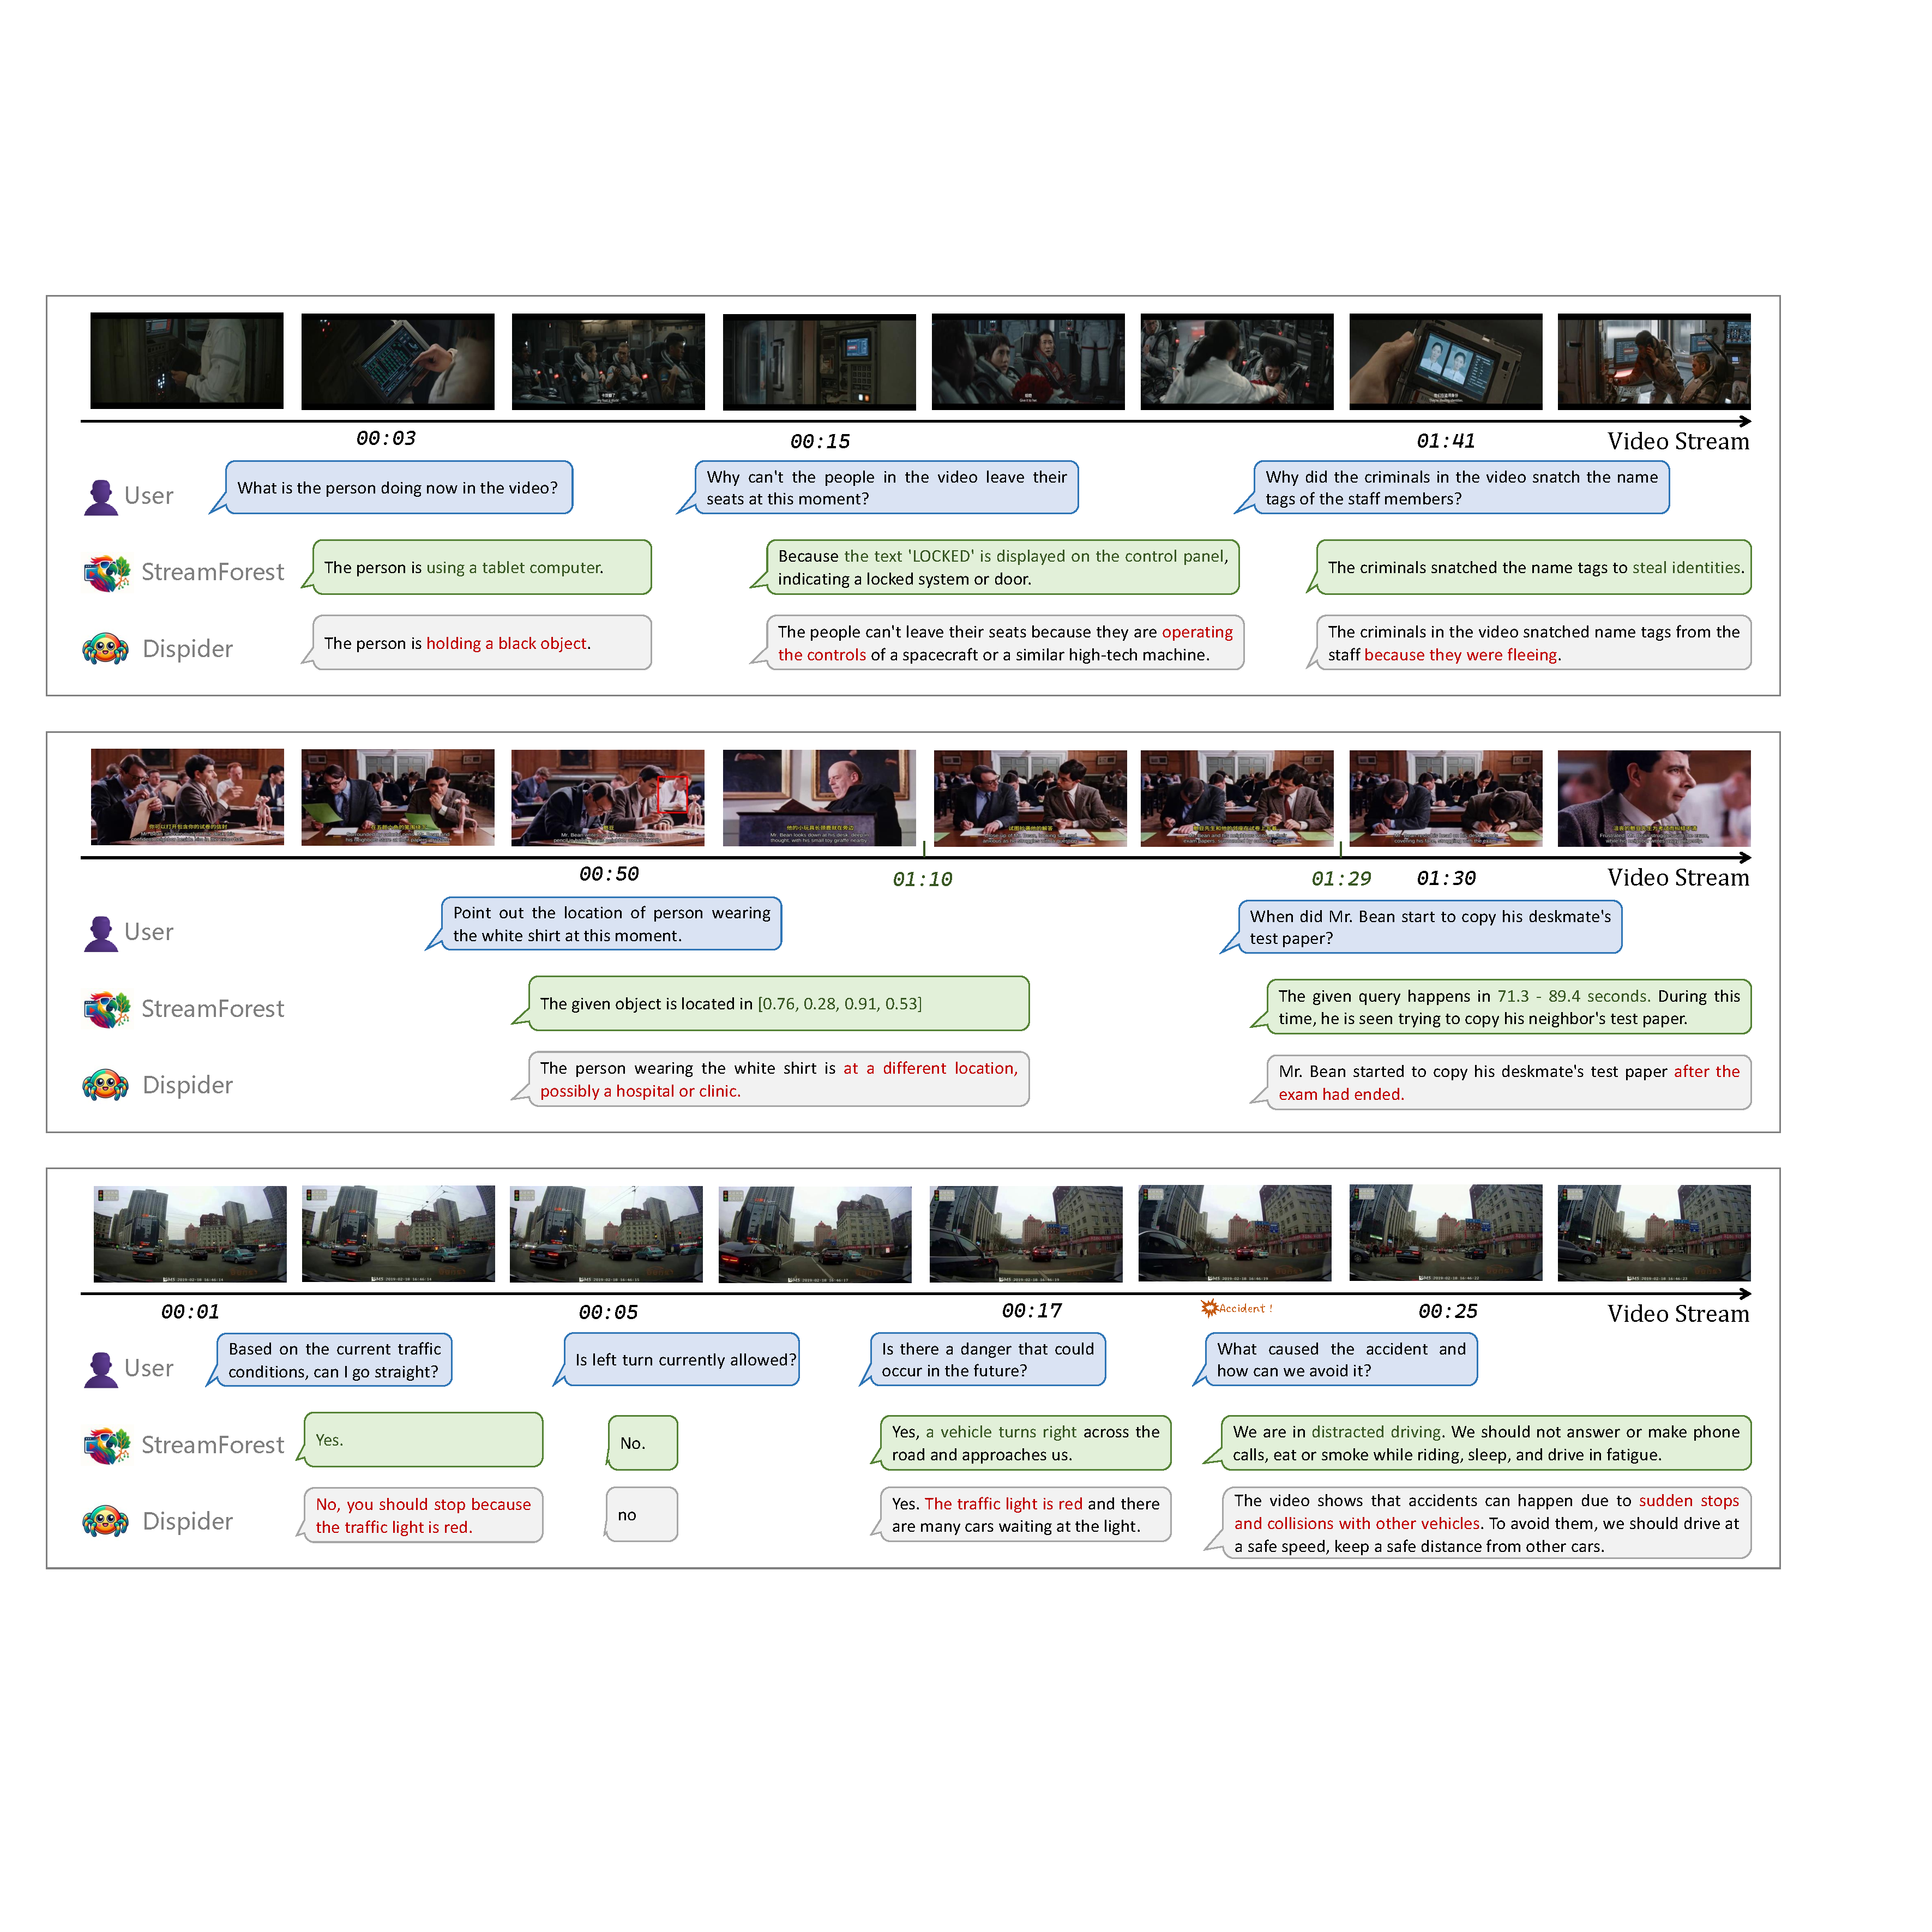
\includegraphics[width=\textwidth]{figs/Appendix/qualitative_comparison_img.pdf} 
    \caption{Comparación cualitativa entre StreamForest y otro método.
    }
    \label{app:fig:qualitative_comparison}
\end{figure*}



Figure \ref{app:fig:qualitative_comparison} presents a qualitative comparison between our model and other method. In the top example, StreamForest demonstrates a superior ability to capture fine-grained visual details and maintain persistent memory over time, enabling more coherent and informed inferences. The middle example highlights StreamForest’s strong spatiotemporal grounding capabilities, accurately localizing objects and events across space and time. The bottom example illustrates the model’s potential in intelligent driving scenarios, where it delivers precise real-time perception and supports future predictions based on both historical and current observations.





\section{More Ablations}
\label{app:sec:More_Ablations}

\begin{figure}[ht]

    \centering
    \begin{minipage}[t]{0.32\textwidth}
        \centering
        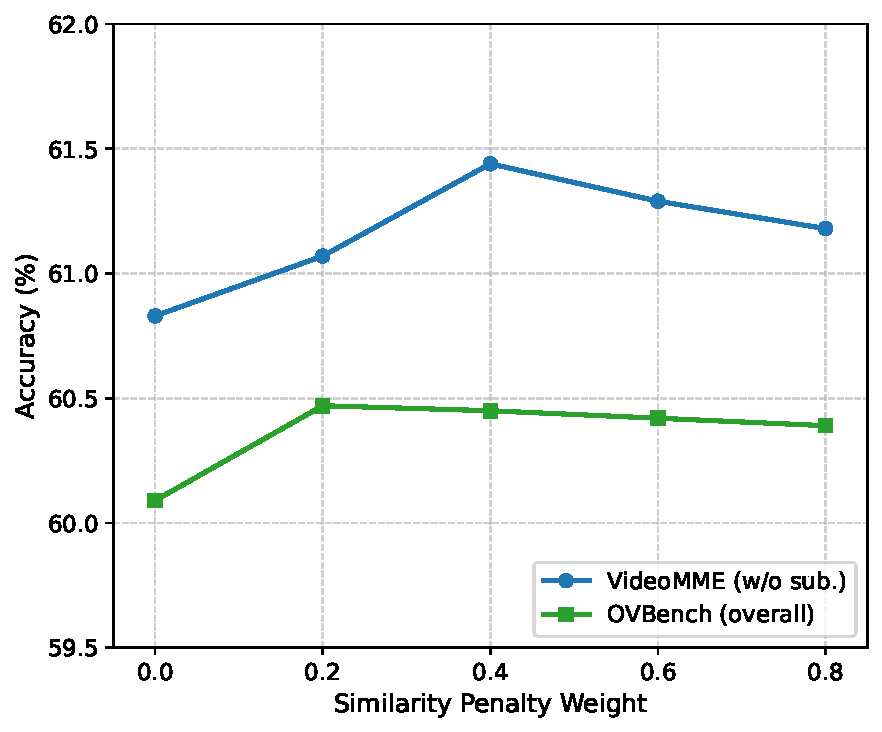
\includegraphics[width=\linewidth]{figs/Appendix/ablation_penalty_similarity.pdf}
    \end{minipage}
    \hfill
    \begin{minipage}[t]{0.32\textwidth}
        \centering
        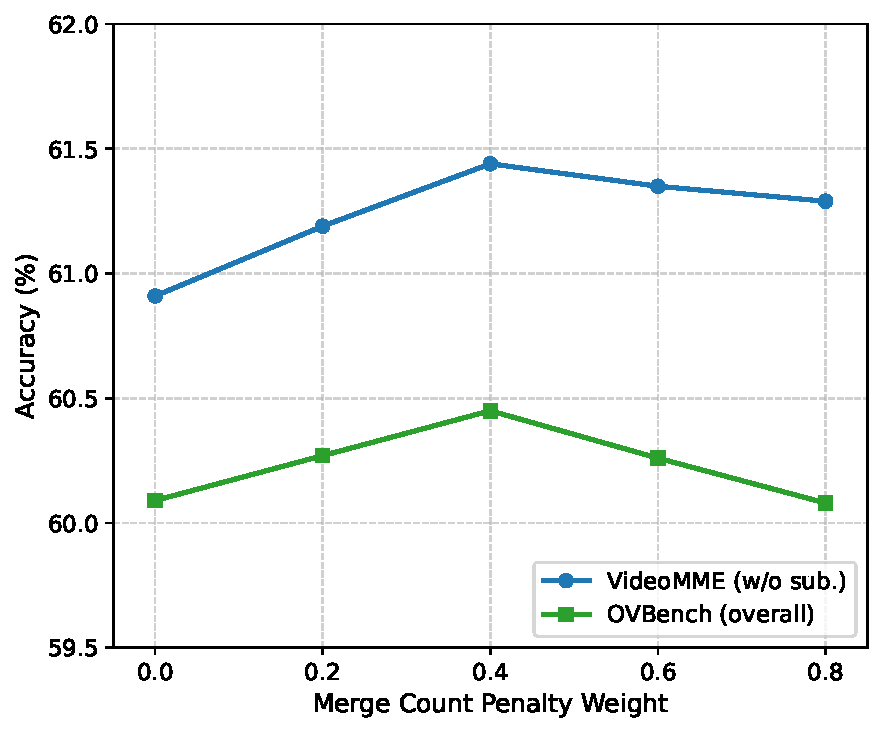
\includegraphics[width=\linewidth]{figs/Appendix/ablation_penalty_mergecount.pdf}
    \end{minipage}
    \hfill
    \begin{minipage}[t]{0.32\textwidth}
        \centering
        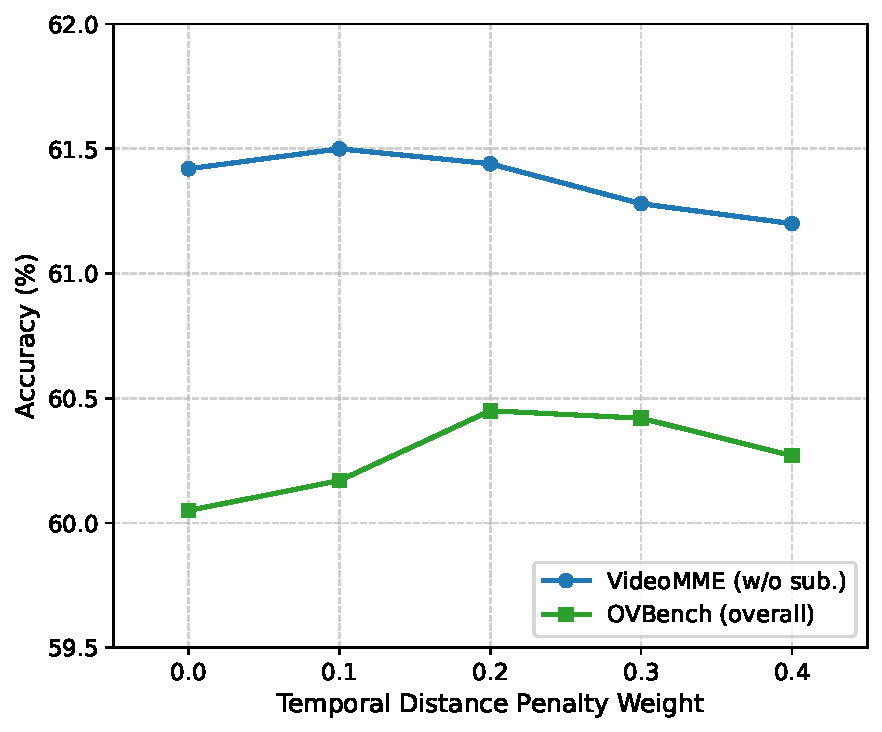
\includegraphics[width=\linewidth]{figs/Appendix/ablation_penalty_temporal.pdf}
    \end{minipage}

    \caption{
        Ablation experiments of three penalty weights.
    }
    \label{app:fig:ablation_penalty_weight}
\end{figure}

To evaluate the effect of each penalty on the effectiveness of long-term memory, we conducted ablation studies by varying the weights of the similarity penalty, merge count penalty, and temporal distance penalty. The results are presented in Figure~\ref{app:fig:ablation_penalty_weight}, which reports the accuracy of both VideoMME and OVBench under different settings. It demonstrates that a balanced combination of penalty weights is more effective. Specifically, 0.4 for both similarity and merge count penalties, and 0.2 for the temporal distance penalty yield the most effective memory construction. This configuration achieves a favorable trade-off between preserving semantic coherence, maintaining diversity in memory representation, and ensuring reasonable temporal continuity.








\section{Efficiency of Multi-round Inference}
\label{app:sec:Efficiency_Multi-round}
We evaluated StreamForest's multi-round response efficiency by streaming a 600-second video to the model at a constant rate of 1 FPS. To isolate processing throughput from text generation latency, the model was constrained to produce a single-token response for each frame. Under this rigorous setting, StreamForest achieved an average processing speed of 9.9 FPS, which is competitive with VideoLLM-Online (12.3 FPS), a model renowned for its real-time capabilities.
Crucially, StreamForest delivers this high efficiency without compromising its substantial superiority in reasoning accuracy over VideoLLM-Online. In stark contrast, Qwen2-VL, another model that also prioritizes reasoning accuracy, demonstrated severe performance bottlenecks. Its processing speed dropped below 1 FPS on a video merely two minutes long, and it encountered out-of-memory (OOM) errors on a single A100-80G GPU after processing only 79 frames.

\begin{table}[h]
    \centering
    \setlength{\tabcolsep}{7pt}
    \renewcommand{\arraystretch}{1.2}
    
    % 
    \caption{Comparison of multi-round inference speed.}
    
    \resizebox{0.5\textwidth}{!}{%
    
    \begin{tabular}{l|cc}
    \toprule
    Method & Resolution & FPS \\ \midrule
    Qwen2.5-VL & 384 & OOM \\
    VideoLLM-Online & 384 & 12.3 \\
    StreamForest (1k) & 384 & 9.9 \\ \bottomrule
    \end{tabular}
        
    }
    
    \label{app:tab:efficiency_multiround}
\end{table}



\section{Discussions}
\label{app:sec:Discussions}
\subsection{Limitations}
\label{app:sec:Discussions:Limitations}

Despite the effectiveness of our proposed method, several limitations remain that warrant further investigation.
%
Our approach can only rely on computing inter-frame similarity to determine moments when the model should proactively produce outputs. Specifically, the method identifies local minima in similarity scores to detect transitions. However, this technique primarily captures coarse scene changes and often fails to accurately detect true semantic event boundaries. To address this limitation, one possible solution is to incorporate a lightweight MLLM as an auxiliary reminder module. This module could provide semantic-level guidance to support more precise and context-aware output decisions.
%
These limitations suggest promising directions for future work.


\subsection{Broader Impacts}
\label{app:sec:Discussions:Broader Impacts}

Our proposed method shows strong potential for real-world streaming video understanding, especially in critical applications like autonomous driving. With domain-specific fine-tuning, it can be adapted to various downstream tasks that require continuous visual processing. As shown in the main text, the model performs well in autonomous driving scenarios, where accurate and timely perception is crucial for safety and decision-making. It can efficiently process live video streams while preserving fine-grained perception and long-term contextual memory. This capability is particularly valuable under limited computational resources, helping improve the reliability and responsiveness of intelligent systems in dynamic environments.

However, as with many vision-language models, potential negative social impacts must also be considered. If deployed without proper safeguards, models may inherit or amplify biases present in training data, leading to unreliable behavior. For instance, performance disparities across different environments or conditions (e.g., weather, lighting, or geographic location) could affect the robustness of StreamForest. To mitigate such risks, we should explore techniques for enhancing interpretability and controllability of streaming video models in safety contexts.




\clearpage
{
\small
\bibliographystyle{plainnat}
\bibliography{reference}
}




\end{document}
